\documentclass{standalone}
\usepackage{tikz}
\usetikzlibrary{patterns, positioning}


\begin{document}
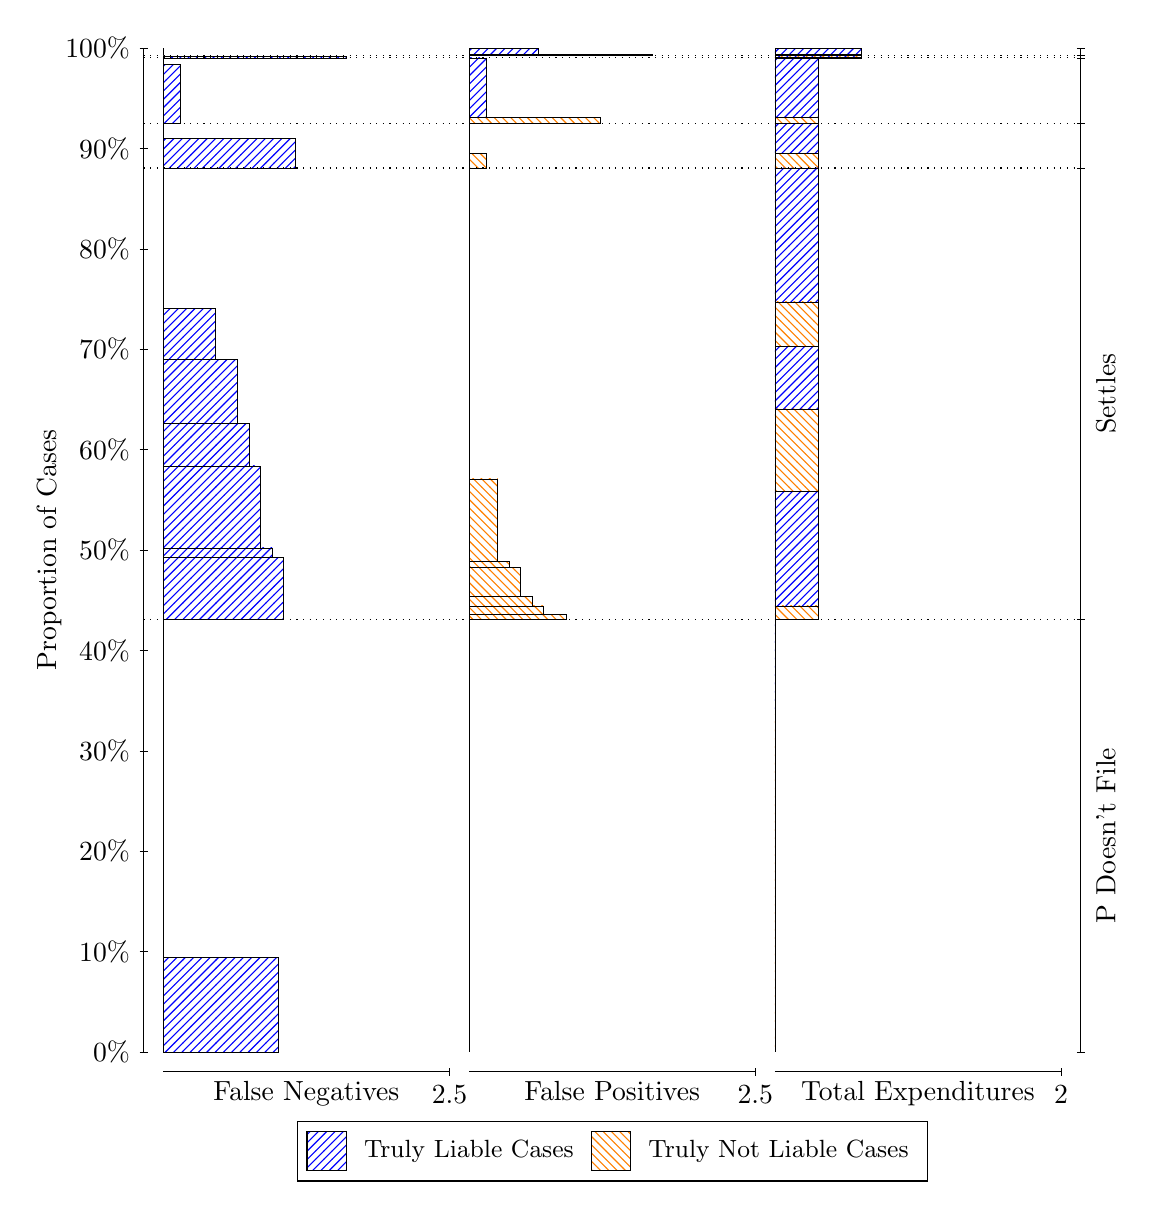
\begin{tikzpicture}
\draw[black, very thin] (1.5,1.75) -- (1.5,14.5);
\node[rotate=90, text=black, anchor=center] at (0.3, 8.125) {Proportion of Cases};
\draw[black, very thin] (1.45,1.75) -- (1.55,1.75);
\node[text=black, anchor=east] at (1.45, 1.75) {0\%};
\draw[black, very thin] (1.45,3.025) -- (1.55,3.025);
\node[text=black, anchor=east] at (1.45, 3.025) {10\%};
\draw[black, very thin] (1.45,4.3) -- (1.55,4.3);
\node[text=black, anchor=east] at (1.45, 4.3) {20\%};
\draw[black, very thin] (1.45,5.575) -- (1.55,5.575);
\node[text=black, anchor=east] at (1.45, 5.575) {30\%};
\draw[black, very thin] (1.45,6.85) -- (1.55,6.85);
\node[text=black, anchor=east] at (1.45, 6.85) {40\%};
\draw[black, very thin] (1.45,8.125) -- (1.55,8.125);
\node[text=black, anchor=east] at (1.45, 8.125) {50\%};
\draw[black, very thin] (1.45,9.4) -- (1.55,9.4);
\node[text=black, anchor=east] at (1.45, 9.4) {60\%};
\draw[black, very thin] (1.45,10.675) -- (1.55,10.675);
\node[text=black, anchor=east] at (1.45, 10.675) {70\%};
\draw[black, very thin] (1.45,11.95) -- (1.55,11.95);
\node[text=black, anchor=east] at (1.45, 11.95) {80\%};
\draw[black, very thin] (1.45,13.225) -- (1.55,13.225);
\node[text=black, anchor=east] at (1.45, 13.225) {90\%};
\draw[black, very thin] (1.45,14.5) -- (1.55,14.5);
\node[text=black, anchor=east] at (1.45, 14.5) {100\%};

\draw[black, very thin] (13.4,1.75) -- (13.4,14.5);
\draw[black, very thin] (13.35,1.75) -- (13.45,1.75);
\node[anchor=west] at (13.35, 1.75) {};
\draw[black, very thin] (13.35,7.2422) -- (13.45,7.2422);
\node[anchor=west] at (13.35, 7.2422) {};
\draw[black, very thin] (13.35,12.977) -- (13.45,12.977);
\node[anchor=west] at (13.35, 12.977) {};
\draw[black, very thin] (13.35,13.541) -- (13.45,13.541);
\node[anchor=west] at (13.35, 13.541) {};
\draw[black, very thin] (13.35,14.375) -- (13.45,14.375);
\node[anchor=west] at (13.35, 14.375) {};
\draw[black, very thin] (13.35,14.404) -- (13.45,14.404);
\node[anchor=west] at (13.35, 14.404) {};
\draw[black, very thin] (13.35,14.5) -- (13.45,14.5);
\node[anchor=west] at (13.35, 14.5) {};

\draw[black, very thin, pattern color=blue, pattern=north east lines] (1.75,1.75) rectangle (3.2033,2.9519);
\draw[black, very thin, pattern color=orange, pattern=north west lines] (1.75,2.9519) rectangle (1.75,7.2422);
\draw[black, very thin, pattern color=blue, pattern=north east lines] (1.75,7.2422) rectangle (3.276,8.0348);
\draw[black, very thin, pattern color=blue, pattern=north east lines] (1.75,8.0348) rectangle (3.1307,8.1527);
\draw[black, very thin, pattern color=blue, pattern=north east lines] (1.75,8.1527) rectangle (2.9853,9.1942);
\draw[black, very thin, pattern color=blue, pattern=north east lines] (1.75,9.1942) rectangle (2.84,9.7353);
\draw[black, very thin, pattern color=blue, pattern=north east lines] (1.75,9.7353) rectangle (2.6947,10.546);
\draw[black, very thin, pattern color=blue, pattern=north east lines] (1.75,10.546) rectangle (2.404,11.191);
\draw[black, very thin, pattern color=orange, pattern=north west lines] (1.75,11.191) rectangle (1.75,12.977);
\draw[black, very thin, pattern color=blue, pattern=north east lines] (1.75,12.977) rectangle (3.4213,13.355);
\draw[black, very thin, pattern color=orange, pattern=north west lines] (1.75,13.355) rectangle (1.75,13.541);
\draw[black, very thin, pattern color=blue, pattern=north east lines] (1.75,13.541) rectangle (1.968,14.292);
\draw[black, very thin, pattern color=orange, pattern=north west lines] (1.75,14.292) rectangle (1.75,14.375);
\draw[black, very thin, pattern color=blue, pattern=north east lines] (1.75,14.375) rectangle (4.0753,14.391);
\draw[black, very thin, pattern color=orange, pattern=north west lines] (1.75,14.391) rectangle (1.75,14.404);
\draw[black, very thin, pattern color=orange, pattern=north west lines] (1.75,14.404) rectangle (1.75,14.421);
\draw[black, very thin, pattern color=blue, pattern=north east lines] (1.75,14.421) rectangle (1.75,14.5);
\draw[black, very thin, pattern color=orange, pattern=north west lines] (5.6333,1.75) rectangle (5.6333,6.0403);
\draw[black, very thin, pattern color=blue, pattern=north east lines] (5.6333,6.0403) rectangle (5.6333,7.2422);
\draw[black, very thin, pattern color=orange, pattern=north west lines] (5.6333,7.2422) rectangle (6.8687,7.3036);
\draw[black, very thin, pattern color=orange, pattern=north west lines] (5.6333,7.3036) rectangle (6.578,7.4141);
\draw[black, very thin, pattern color=orange, pattern=north west lines] (5.6333,7.4141) rectangle (6.4327,7.5342);
\draw[black, very thin, pattern color=orange, pattern=north west lines] (5.6333,7.5342) rectangle (6.2873,7.9061);
\draw[black, very thin, pattern color=orange, pattern=north west lines] (5.6333,7.9061) rectangle (6.142,7.9808);
\draw[black, very thin, pattern color=orange, pattern=north west lines] (5.6333,7.9808) rectangle (5.9967,9.0289);
\draw[black, very thin, pattern color=blue, pattern=north east lines] (5.6333,9.0289) rectangle (5.6333,12.977);
\draw[black, very thin, pattern color=orange, pattern=north west lines] (5.6333,12.977) rectangle (5.8513,13.163);
\draw[black, very thin, pattern color=blue, pattern=north east lines] (5.6333,13.163) rectangle (5.6333,13.541);
\draw[black, very thin, pattern color=orange, pattern=north west lines] (5.6333,13.541) rectangle (7.3047,13.624);
\draw[black, very thin, pattern color=blue, pattern=north east lines] (5.6333,13.624) rectangle (5.8513,14.375);
\draw[black, very thin, pattern color=orange, pattern=north west lines] (5.6333,14.375) rectangle (5.6333,14.388);
\draw[black, very thin, pattern color=blue, pattern=north east lines] (5.6333,14.388) rectangle (5.6333,14.404);
\draw[black, very thin, pattern color=orange, pattern=north west lines] (5.6333,14.404) rectangle (7.9587,14.421);
\draw[black, very thin, pattern color=blue, pattern=north east lines] (5.6333,14.421) rectangle (6.5053,14.5);
\draw[black, very thin, pattern color=orange, pattern=north west lines] (9.5167,1.75) rectangle (9.5167,6.0403);
\draw[black, very thin, pattern color=blue, pattern=north east lines] (9.5167,6.0403) rectangle (9.5167,7.2422);
\draw[black, very thin, pattern color=orange, pattern=north west lines] (9.5167,7.2422) rectangle (10.062,7.4141);
\draw[black, very thin, pattern color=blue, pattern=north east lines] (9.5167,7.4141) rectangle (10.062,8.8694);
\draw[black, very thin, pattern color=orange, pattern=north west lines] (9.5167,8.8694) rectangle (10.062,9.9176);
\draw[black, very thin, pattern color=blue, pattern=north east lines] (9.5167,9.9176) rectangle (10.062,10.71);
\draw[black, very thin, pattern color=orange, pattern=north west lines] (9.5167,10.71) rectangle (10.062,11.277);
\draw[black, very thin, pattern color=blue, pattern=north east lines] (9.5167,11.277) rectangle (10.062,12.977);
\draw[black, very thin, pattern color=orange, pattern=north west lines] (9.5167,12.977) rectangle (10.062,13.163);
\draw[black, very thin, pattern color=blue, pattern=north east lines] (9.5167,13.163) rectangle (10.062,13.541);
\draw[black, very thin, pattern color=orange, pattern=north west lines] (9.5167,13.541) rectangle (10.062,13.624);
\draw[black, very thin, pattern color=blue, pattern=north east lines] (9.5167,13.624) rectangle (10.062,14.375);
\draw[black, very thin, pattern color=orange, pattern=north west lines] (9.5167,14.375) rectangle (10.607,14.388);
\draw[black, very thin, pattern color=blue, pattern=north east lines] (9.5167,14.388) rectangle (10.607,14.404);
\draw[black, very thin, pattern color=orange, pattern=north west lines] (9.5167,14.404) rectangle (10.607,14.421);
\draw[black, very thin, pattern color=blue, pattern=north east lines] (9.5167,14.421) rectangle (10.607,14.5);
\draw[black, dotted] (1.5,7.2422) -- (13.4,7.2422);
\draw[black, dotted] (1.5,12.977) -- (13.4,12.977);
\draw[black, dotted] (1.5,13.541) -- (13.4,13.541);
\draw[black, dotted] (1.5,14.375) -- (13.4,14.375);
\draw[black, dotted] (1.5,14.404) -- (13.4,14.404);
\draw[black, very thin] (1.75,1.5) -- (5.3833,1.5);
\node[text=black, anchor=north] at (3.5667, 1.5) {False Negatives};
\draw[black, very thin] (5.3833,1.45) -- (5.3833,1.55);
\node[text=black, anchor=north] at (5.3833, 1.45) {2.5};

\draw[black, very thin] (5.6333,1.5) -- (9.2667,1.5);
\node[text=black, anchor=north] at (7.45, 1.5) {False Positives};
\draw[black, very thin] (9.2667,1.45) -- (9.2667,1.55);
\node[text=black, anchor=north] at (9.2667, 1.45) {2.5};

\draw[black, very thin] (9.5167,1.5) -- (13.15,1.5);
\node[text=black, anchor=north] at (11.333, 1.5) {Total Expenditures};
\draw[black, very thin] (13.15,1.45) -- (13.15,1.55);
\node[text=black, anchor=north] at (13.15, 1.45) {2};

\node[text=black, centered, rotate=90] at (13.72, 4.4961) {P Doesn't File};
\node[text=black, centered, rotate=90] at (13.72, 10.11) {Settles};





\draw (7.449999999999999,1.5) node[draw=none] (baseCoordinate) {};
\begin{scope}[align=center]
        \matrix[scale=0.5, draw=black, below=0.5cm of baseCoordinate, nodes={draw}, column sep=0.1cm]{
            \node[rectangle, draw, minimum width=0.5cm, minimum height=0.5cm, pattern color=blue, pattern=north east lines] {}; &
            \node[draw=none, font=\small, text=black] (B) {Truly Liable Cases}; &
            \node[rectangle, draw, minimum width=0.5cm, minimum height=0.5cm, pattern color=orange, pattern=north west lines] {}; &
            \node[draw=none, font=\small, text=black] (B) {Truly Not Liable Cases}; \\
            };
\end{scope}

\end{tikzpicture}
\end{document}